\documentclass[12pt,a4paper]{article}
\usepackage[T1]{fontenc}
\usepackage{lmodern,amsmath,amssymb,booktabs,enumitem}
\usepackage[margin=21mm,top=18mm,bottom=19mm]{geometry}
\usepackage{xcolor,tikz}
\definecolor{course}{HTML}{982A32}
\definecolor{bluemode}{HTML}{205C7A}
\setlength{\parindent}{0pt}
\setlength{\parskip}{4pt}
\setlist[enumerate]{label=\textbf{\alph*)},leftmargin=1.8em,itemsep=5pt,topsep=3pt,parsep=0pt}
\newcommand{\T}{^{\mathsf T}}
\newcommand{\bK}{\overline{\mathbf K}}
\newcommand{\bM}{\overline{\mathbf M}}
\newcommand{\vct}[1]{\mathbf{#1}}
\newcommand{\colv}[1]{\begin{bmatrix}#1\end{bmatrix}}
\newcommand{\coursehead}[1]{%
  {\small ME473 -- Dynamic finite element analysis of structures\hfill EPFL\\
  Stefano Burzio\hfill 2026\par}
  \vspace{3mm}\begin{center}\Large\bfseries #1\end{center}
  \vspace{-2mm}{\color{course}\hrule height 0.7pt}\vspace{2mm}}
\newcommand{\ptitle}[1]{\vspace{2mm}{\large\bfseries #1\par}\vspace{1mm}}
\newcommand{\subpart}[1]{\smallskip{\bfseries #1}\ }
\raggedbottom

\begin{document}
\coursehead{Problem set 10 -- Solutions}
\ptitle{Problem 1 \quad Full five-node reference}
\subpart{a) Element assembly.}
For the nodal twist on one element, the two linear shape functions have
derivatives $-1/h$ and $1/h$. Integration of the stiffness and inertia terms
gives
\[
 \vct K_e=\frac{GI_p}{h}\colv{1&-1\\-1&1},
 \qquad \vct M_e=\frac{\rho I_ph}{6}\colv{2&1\\1&2}.
\]
Each interior node belongs to two elements. Each free end belongs to one.
Assembling and scaling with $h=\ell/4$ gives
\[
 \bK=4\colv{1&-1&0&0&0\\-1&2&-1&0&0\\0&-1&2&-1&0\\
                0&0&-1&2&-1\\0&0&0&-1&1},\qquad
 \bM=\frac1{24}\colv{2&1&0&0&0\\1&4&1&0&0\\0&1&4&1&0\\
                    0&0&1&4&1\\0&0&0&1&2}.
\]
Every row of $\bK$ sums to zero. A rigid rotation therefore has zero strain
energy and zero frequency. The total dimensionless mass is
$\vct1\T\bM\vct1=1$.

\subpart{Exact eigenpairs of the discrete model.}
Set $\theta_k=k\pi/4$ and $p^{(k)}_j=\cos(j\theta_k)$, $j=0,\ldots,4$.
For an interior row, the sum of adjacent entries is
$2\cos(\theta_k)p^{(k)}_j$. Substitution in the full pencil gives
\[
 \Lambda_k^{\rm FE}=96\,\frac{1-\cos\theta_k}{2+\cos\theta_k},
 \qquad \Omega_k^{\rm FE}=\sqrt{\Lambda_k^{\rm FE}},\qquad k=0,\ldots,4 .
\]
The left endpoint row gives the same ratio. At the right endpoint,
$\sin(4\theta_k)=0$ supplies the corresponding endpoint relation.

\begin{center}
\begin{tabular}{@{}crrrl@{}}
\toprule
$k$ & $\Lambda^{\rm FE}_k$ & $\Omega^{\rm FE}_k$ & $\Omega_k^{\rm cont}$ &
Nodal shape, left end $=1$\\
\midrule
0 & 0         & 0         & 0         & $(1,1,1,1,1)$\\
1 & 10.386642 & 3.222831  & 3.141593  & $(1,a,0,-a,-1)$\\
2 & 48        & 6.928203  & 6.283185  & $(1,0,-1,0,1)$\\
3 & 126.756215& 11.258606 & 9.424778  & $(1,-a,0,a,-1)$\\
4 & 192       & 13.856406 & 12.566371 & $(1,-1,1,-1,1)$\\
\bottomrule
\end{tabular}\\[-1pt]
{\small $a=1/\sqrt2$. Multiply $\Omega$ by $\sqrt{G/\rho}/\ell$ to recover
$\omega$ in rad/s.}
\end{center}
The continuum equation $GI_p\varphi''+\rho I_p\omega^2\varphi=0$ with
$\varphi'(0)=\varphi'(\ell)=0$ gives $\varphi_k(x)=\cos(k\pi x/\ell)$.
On this uniform mesh, its nodal samples agree with the exact FE eigenvectors.
Between nodes, each FE shape is piecewise linear. For $k=1$ the FE frequency
exceeds the continuum frequency by $2.5859\%$.

\newpage
\ptitle{Problem 1 \quad What each trial space can represent}
\subpart{b) Projection and recovery.}
Stationarity of the Rayleigh quotient on $\vct p=\vct\Psi\vct y$ gives
$\vct\Psi\T(\bK\vct\Psi\vct y-\widehat\Lambda\bM\vct\Psi\vct y)=\vct0$.
For $\vct\Psi_g$ this reduces to
\[
 \vct K^*=\colv{0&0\\0&1168},\qquad
 \vct M^*=\colv{1&0\\0&337/3},\qquad
 \widehat\Lambda_0=0,\qquad \widehat\Lambda_1=\frac{3504}{337}.
\]
The reduced eigenvectors are $\vct e_1$ and $\vct e_2$. At unit left-end
amplitude, the lifted shapes are
\[
 \widehat{\vct p}_0=(1,1,1,1,1)\T,\qquad
 \widehat{\vct p}_1=(1,11/16,0,-11/16,-1)\T .
\]

\subpart{c) Errors for the target modes.}
The constant column reproduces rigid rotation exactly. For the elastic
mode the interior amplitudes are $0.6875$ and $-0.6875$, compared with
$\pm1/\sqrt2$ in the full FE mode. The resulting errors are
\begin{center}
\begin{tabular}{@{}lrrr@{}}
\toprule
Reference for $k=1$ & Reference $\Omega_1$ &
Error in $\widehat\Lambda_1$ & Error in $\widehat\Omega_1$\\
\midrule
Full five-node FE & $3.222831$ & $0.10575\%$ & $0.05286\%$\\
Exact continuum   & $3.141593$ & $5.34998\%$ & $2.64014\%$\\
\bottomrule
\end{tabular}
\end{center}
The Ritz estimate is $\widehat\Omega_1=3.224535$. The one-element result
$\sqrt{12}=3.464102$ was $10.2658\%$ above $\pi$.
Most of the remaining frequency error comes from the mesh. The two MAC
values against the full FE modes are $1$ and $0.999906$.

\subpart{d) A space that misses both targets.}
For the supplied $\vct\Psi_b$,
\[
 \vct K^*=\colv{80&-48\\-48&80},\qquad
 \vct M^*=\tfrac23\vct I,\qquad
 (\widehat\Lambda,\vct y)=(48,(1,1)\T),\ (192,(1,-1)\T).
\]
Their lifted shapes, scaled at the left end, are $(1,0,-1,0,1)\T$ and
$(1,-1,1,-1,1)\T$. These are exactly the full FE modes $k=2,4$.
Every trial vector is symmetric about the midpoint, whereas the first
elastic mode is antisymmetric. Also
$\vct1\T\bM=(1,2,2,2,1)/8$, so $\vct1\T\bM\vct\Psi_b=\vct0$.
Both trial columns are mass-orthogonal to rigid rotation. Consequently every
vector in this space has zero MAC with either target. In increasing order,
the absolute error against $\Lambda_0$ is $48$ and the relative error against
$\Lambda_1$ is $1748.53\%$. Both returned pairs have zero full FE residual:
a residual checks equilibrium for a mode, while mode identification tells us
which frequency was found.

\begin{center}
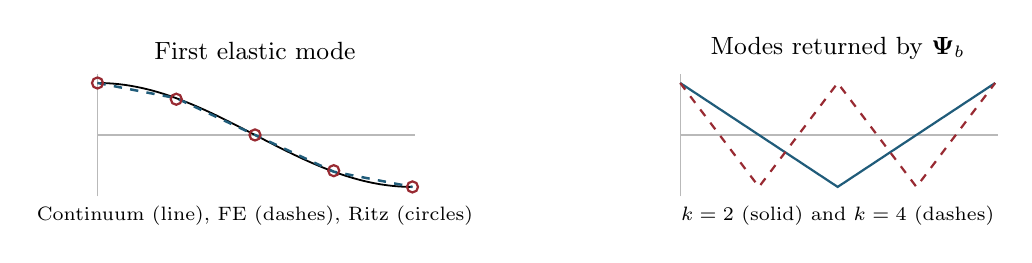
\begin{tikzpicture}[x=1cm,y=1cm,font=\small]
\begin{scope}[xshift=0cm]
 \node[anchor=south] at (2,0.84) {First elastic mode};
 \draw[gray!55] (0,0)--(4.03,0);
 \draw[gray!55] (0,-0.78)--(0,0.78);
 \draw[black,line width=.65pt,domain=0:4,samples=61,smooth] plot (\x,{0.66*cos(45*\x)});
 \draw[bluemode,line width=.9pt,dashed] (0,.66)--(1,.46669)--(2,0)--(3,-.46669)--(4,-.66);
 \foreach \x/\y in {0/.66,1/.45375,2/0,3/-.45375,4/-.66}
    \draw[course,thick] (\x,\y) circle(2pt);
 \node[anchor=north] at (2,-.78) {\scriptsize Continuum (line), FE (dashes), Ritz (circles)};
\end{scope}
\begin{scope}[xshift=7.4cm]
 \node[anchor=south] at (2,0.84) {Modes returned by $\vct\Psi_b$};
 \draw[gray!55] (0,0)--(4.03,0);
 \draw[gray!55] (0,-0.78)--(0,0.78);
 \draw[bluemode,thick] (0,.66)--(1,0)--(2,-.66)--(3,0)--(4,.66);
 \draw[course,thick,dashed] (0,.66)--(1,-.66)--(2,.66)--(3,-.66)--(4,.66);
 \node[anchor=north] at (2,-.78) {\scriptsize $k=2$ (solid) and $k=4$ (dashes)};
\end{scope}
\end{tikzpicture}
\end{center}

\subpart{MATLAB implementation.}
The same four lines solve either reduction. Here \texttt{K} and \texttt{M}
denote the dimensionless matrices and \texttt{V} holds the two trial columns.
\begin{verbatim}
Kr = V'*K*V;                    Mr = V'*M*V;
[Y,D] = eig(Kr,Mr);
[lambdaR,idx] = sort(diag(D));
P = V*Y(:,idx);                  % five nodal entries per mode
\end{verbatim}
The companion script \texttt{ProblemSet10\_shaft.m} also assembles the full
matrices, evaluates the errors and plots both target modes.

\newpage
\ptitle{Problem 2 \quad Inverse Lanczos on the three-node bar}
\subpart{a) Operator and inner product.}
In units of $c=E/(\rho\ell^2)$ the unshifted problem is
$2\vct C\vct p=\mu\vct D\vct p$. The product
\[
 \vct D\vct B=\frac1{13}\colv{24&56&11\\56&252&56\\11&56&24}
\]
is symmetric, so $\vct B$ is self-adjoint in the $D$-inner product.
The inverse preserves the mode shape and changes its eigenvalue to
$\nu=14/(\mu+2)$. Hence $\mu_\sigma=14/\nu$ and $\mu=14/\nu-2$.
The largest $\nu$ gives the lowest physical frequency.

\subpart{b) The two steps.}
The starting vector has squared $D$-norm $2^2+4(1)^2=8$. Direct products
with the supplied matrix give
\[
 \vct q_1=\frac{(2,1,0)\T}{\sqrt8},\qquad
 \vct B\vct q_1=\frac{(8,7,6)\T}{\sqrt8},\qquad
 \alpha_1=\frac{2(8)+4(7)}8=\frac{11}{2}.
\]
After this single step the rigid-mode estimate is
$\widehat\mu_0=14/(11/2)-2=6/11$, with trial shape $(1,1/2,0)\T$.
Subtracting the projection gives
\[
 \vct w_1=\frac{3}{2\sqrt8}(-2,1,4)\T,\qquad
 \beta_1=\frac{3\sqrt3}{2},\qquad
 \vct q_2=\frac{(-2,1,4)\T}{\sqrt{24}}.
\]
The second product is $\vct B\vct q_2=(4,7,10)\T/\sqrt{24}$.
Thus $\alpha_2=(-8+28+40)/24=5/2$. Substitution into
$\vct w_2=\vct B\vct q_2-\alpha_2\vct q_2-\beta_1\vct q_1$ gives
$\vct w_2=\vct0$ and $\beta_2=0$.

\subpart{c) Ritz pairs and nodal shapes.}
The projected matrix and its characteristic polynomial are
\[
 \vct T_2=\frac12\colv{11&3\sqrt3\\3\sqrt3&5},\qquad
 \det(\nu\vct I-\vct T_2)=\nu^2-8\nu+7=(\nu-7)(\nu-1).
\]
With $\vct Q_2=[\vct q_1,\vct q_2]$ the two reconstructions are
\begin{center}
\begin{tabular}{@{}cccccl@{}}
\toprule
$\nu$ & $\vct y\T$ & $(\vct Q_2\vct y)\T$ & $\mu_\sigma$ & $\mu$ & Mode\\
\midrule
$7$ & $(\sqrt3,1)/2$ & $(1,1,1)/\sqrt6$ & $2$ & $0$ & Rigid translation\\
$1$ & $(1,-\sqrt3)/2$ & $(1,0,-1)/\sqrt2$ & $14$ & $12$ & First elastic\\
\bottomrule
\end{tabular}
\end{center}
To verify these are exact pairs of the original pencil, observe that
$\vct C(1,1,1)\T=\vct0$ and
$2\vct C(1,0,-1)\T=(12,0,-12)\T=12\vct D(1,0,-1)\T$.
The dimensional eigenvalues are $0$ and $12E/(\rho\ell^2)$, with angular
frequencies $0$ and $\sqrt{12E/\rho}/\ell$.

\newpage
\ptitle{Problem 2 \quad Comparison with subspace iteration}
\subpart{d) Eigenvalue and shape comparisons.}
The shifted eigenvalue makes a relative error well-defined for the rigid
mode. Use $100|\widehat\mu_\sigma-\mu_\sigma|/\mu_\sigma$. With each left
end fixed at unit amplitude for comparison, the largest nodal discrepancy
is $\max_j|\widehat p_j-p_j|$.
\begin{center}
\begin{tabular}{@{}llrrr@{}}
\toprule
Method & Mode & $\widehat\mu_\sigma$ & Shifted error & Largest nodal error\\
\midrule
Exact        & Rigid   & $2$ & -- & --\\
Lanczos, 2 steps & Rigid & $2$ & $0$ & $0$\\
Subspace, 3 iterations & Rigid & $2.000002317$ & $0.000116\%$ & $0.000438$\\
\addlinespace
Exact & First elastic & $14$ & -- & --\\
Lanczos, 2 steps & First elastic & $14$ & $0$ & $0$\\
Subspace, 3 iterations & First elastic & $14.423259$ & $3.0233\%$ & $0.270029$\\
\bottomrule
\end{tabular}
\end{center}
For the rigid mode the largest difference is at the midpoint
($1.000438$ versus $1$). For the first elastic mode it is at the right
end ($-0.729971$ versus $-1$). Subtracting $2$ from the subspace values
gives the unshifted estimates $0.000002317$ and $12.423259$.

\subpart{Why two steps suffice here.}
Write the starting vector as
\[
 (2,1,0)\T=(1,1,1)\T+(1,0,-1)\T .
\]
Both components are exact modes, and their inverse eigenvalues are distinct.
Consequently $\vct q_1$ and $\vct B\vct q_1$ span exactly those two modes.
The vanishing $\beta_2$ records that applying $\vct B$ cannot produce a
third independent direction. The third mode $(2,-1,2)\T$, with $\mu=24$,
is $D$-orthogonal to the start.

The initial block $[\vct e_1,\vct e_2]$ in Problem Set 9 has a component
in this third mode. Each shifted inverse iteration multiplies the first
elastic component relative to the third by $26/14$, and the rigid
component relative to the third by $26/2$. This explains why the rigid
mode is already much more accurate after three iterations. The exact
two-step Lanczos result depends on the chosen starting shape.

\subpart{Reproducing the supplied subspace reference.}
For instructors, the three-step result can also be constructed from a single
two-column basis. Put $\vct H=2\vct C+2\vct D$ and set
\[
 \vct U=(\vct H^{-1}\vct D)^3[\vct e_1,\vct e_2].
\]
The intermediate Ritz extractions change the basis within each block.
Thus the final trial space is $\operatorname{range}(\vct U)$. Solve
$(\vct U\T\vct H\vct U)\vct y
=\widehat\mu_\sigma(\vct U\T\vct D\vct U)\vct y$ and rescale
$\vct U\vct y$ by its first entry. The resulting nodal shapes are
$(1,1.000438,0.999603)\T$ and $(1,-0.067550,-0.729971)\T$.
\newpage
\ptitle{Problem 3 \quad Choosing a Jacobi pivot}
\subpart{a) The sign of the standard rotation.}
Write $c_\theta=\cos\theta$, $s_\theta=\sin\theta$.
The rotated off-diagonal entry is the stiffness product of the first
and second columns of $\vct R$:
\begin{align*}
 k'_{ij}
 &= (c_\theta,s_\theta)\vct K_p(-s_\theta,c_\theta)\T\\
 &=k_{ij}(c_\theta^2-s_\theta^2)
    -(k_{ii}-k_{jj})c_\theta s_\theta\\
 &=k_{ij}\cos(2\theta)-\tfrac12(k_{ii}-k_{jj})\sin(2\theta).
\end{align*}
Setting $k'_{ij}=0$ gives, for a nonzero pivot and unequal diagonal entries,
\[
 \boxed{\displaystyle \tan(2\theta)=\frac{2k_{ij}}{k_{ii}-k_{jj}}.}
\]
Choose $2\theta$ from the principal arctangent branch. This selects
$|\theta|<\pi/4$ and avoids exchanging the pivot axes by a large rotation.
If $k_{ij}=0$, take $\theta=0$. If $k_{ii}=k_{jj}$ and $k_{ij}\ne0$,
take $\theta=\pi/4$; then $\cos(2\theta)=0$. In all cases
$|\theta|\leq\pi/4$ and $\vct R\T\vct I\vct R=\vct I$.

\subpart{b) The two conditions for a generalized pivot.}
The columns are $\vct u=(1,\gamma)\T$ and $\vct v=(\alpha,1)\T$.
For any symmetric pivot block $\vct A_p$,
\[
 \vct u\T\vct A_p\vct v
 = a_{ii}\alpha+a_{jj}\gamma+a_{ij}(1+\alpha\gamma).
\]
Applying this product to $\vct K_p$ and $\vct M_p$ and setting each result
to zero gives the two equations in the question. Symmetry clears the
transposed entries as well.

\subpart{c) Elimination and root choice.}
Denote the two pivot equations by $F_K=0$ and $F_M=0$, in the order given.
The combination $m_{ij}F_K-k_{ij}F_M$ gives
$\bar k_{ii}\alpha+\bar k_{jj}\gamma=0$. Two other combinations,
$m_{jj}F_K-k_{jj}F_M$ and $k_{ii}F_M-m_{ii}F_K$, give
\[
 2\bar k\,\alpha=\bar k_{jj}(1+\alpha\gamma),\qquad
 2\bar k\,\gamma=-\bar k_{ii}(1+\alpha\gamma).
\]
Write $\alpha=\bar k_{jj}/x$ and $\gamma=-\bar k_{ii}/x$. Since
$1+\alpha\gamma=1-\bar k_{ii}\bar k_{jj}/x^2$, substitution gives
\[
 x^2-2\bar k\,x-\bar k_{ii}\bar k_{jj}=0,\qquad
 x_\pm=\bar k\pm\sqrt{\bar k^2+\bar k_{ii}\bar k_{jj}} .
\]
The larger-magnitude root adds terms of the same sign, avoiding
subtractive cancellation. For a nondegenerate pivot this gives
\[
 \boxed{\displaystyle
 x=\bar k+\operatorname{sgn}(\bar k)
       \sqrt{\bar k^2+\bar k_{ii}\bar k_{jj}},\qquad
 \alpha=\frac{\bar k_{jj}}{x},\qquad
 \gamma=-\frac{\bar k_{ii}}{x}.}
\]

\newpage
\ptitle{Problem 3 \quad Limiting cases and a numerical check}
\subpart{The sign at a tie.}
When $\bar k=0$ and the radicand is positive, the roots have equal
magnitude. Take the positive root, equivalently $\operatorname{sgn}(0)=+1$
for this root-selection rule. An already diagonal pair needs no update.
If all three barred quantities vanish for a coupled pivot, the blocks are
proportional. In this case take $\gamma=0$ and
$\alpha=-m_{ij}/m_{ii}$. This diagonalizes $\vct M_p$ and its multiple
$\vct K_p$ without dividing by $x=0$.

\subpart{Recovering the standard rotation.}
For $\vct M_p=\vct I$, the mass equation gives $\alpha=-\gamma$.
Putting $t=\gamma$ leaves the stiffness equation
\[
 (k_{ii}-k_{jj})t=k_{ij}(1-t^2).
\]
The columns have the same length $\sqrt{1+t^2}$. Normalizing both gives
\[
 \frac{1}{\sqrt{1+t^2}}\colv{1&-t\\t&1}
 =\colv{\cos\theta&-\sin\theta\\\sin\theta&\cos\theta},
 \qquad t=\tan\theta .
\]
For $|t|<1$, the identity $\tan(2\theta)=2t/(1-t^2)$ gives the formula
in part (a). With equal diagonals and a nonzero pivot, $t=\pm1$ gives the
endpoint rotations $\theta=\pm\pi/4$.

\subpart{d) A numerical pivot.}
For the given stiffness block, $\tan(2\theta)=-1/2$.
The small-angle branch has $\cos(2\theta)=2/\sqrt5$ and
$\sin(2\theta)=-1/\sqrt5$. It clears the stiffness pivot, but the rotated
mass still has the off-diagonal entry
\[
 m'_{ij}=m_{ij}\cos(2\theta)-\tfrac12(m_{ii}-m_{jj})\sin(2\theta)
        =\frac{2}{\sqrt5}-\frac{3}{2\sqrt5}=\frac{1}{2\sqrt5}.
\]
For the generalized transformation the intermediate quantities are
\[
 \bar k_{ii}=3(1)-1(1)=2,\qquad
 \bar k_{jj}=7(1)-4(1)=3,\qquad
 \bar k=\tfrac12[3(4)-7(1)]=\tfrac52 .
\]
The square root is $7/2$, so $x=6$ and
\[
 \boxed{\alpha=\tfrac12,\qquad\gamma=-\tfrac13},\qquad
 \vct J=\colv{1&1/2\\-1/3&1}.
\]
Here $\det\vct J=7/6$. Direct multiplication gives
\[
 \vct J\T\vct K_p\vct J=\colv{28/9&0\\0&35/4},\qquad
 \vct J\T\vct M_p\vct J=\colv{7/9&0\\0&21/4}.
\]
The diagonal ratios are $4$ and $5/3$, respectively. The corresponding
columns of $\vct J$ are eigenvectors of the original pencil. As an
independent check, $\det(\vct K_p-\lambda\vct M_p)
=3\lambda^2-17\lambda+20=(\lambda-4)(3\lambda-5)$.
\end{document}
